\setAuthor{}
\setRound{piirkonnavoor}
\setYear{2020}
\setNumber{G 10}
\setDifficulty{10}
\setTopic{TODO}

\prob{Teleskoop}
On antud 4 ühesugust õhukest kumerläätse fookuskaugusega $f$ ning toru pikkusega $12f$ mille siseläbimõõt ühtib läätse välisläbimõõduga. Leidke maksimaalne suurendus teleskoobile mille saab ehitada nendest komponetidest. Lisage optiline skeem. 
\emph{Märkus:} Teleskoop on optiline seade, mille sisenevad ja väljuvad kiired on paralleelsed. Teleskoobi suurenduseks nimetatakse nurksuurendust $ \beta = {\alpha}_{2} / {\alpha}_{1}$, kus $\alpha_1$ on nurk mille all paistab ese vaatleja jaoks ilma teleskoobita ja $\alpha_2$ on nurk mille all paistab eseme kujutis teleskoobis. (Näiteks kahe läätse puhul $ \beta = f_1 / f_2 $.)



\hint

\solu
Kui koostaksime teleskoobi vaid kahest komponendist siis nurksuurenduse saamiseks peame eelkõige tekitama olukorra kus optiliste komponentide fookuskaugused on erinevad.
Kõrvuti asetatud õhukeste läätsede optilised tugevused liituvad. Kahe läätse liitmisel saame seega läätse fookuskaugusega $ \frac{f}{2} $ ja kui asetaksime kolm läätse kõrvuti siis ühendläätse fookuskauguseks kujuneks $ \frac{f}{3} $

\vspace{20pt}
\emph{Variant 1}\\
\textbf{Teleskoop mis koosneks siis ühest üksikust läätsest ja ühest kaheläätselisest komponendist annaks suurenduse 2 korda.}

\vspace{-10pt}
  \begin{center}
    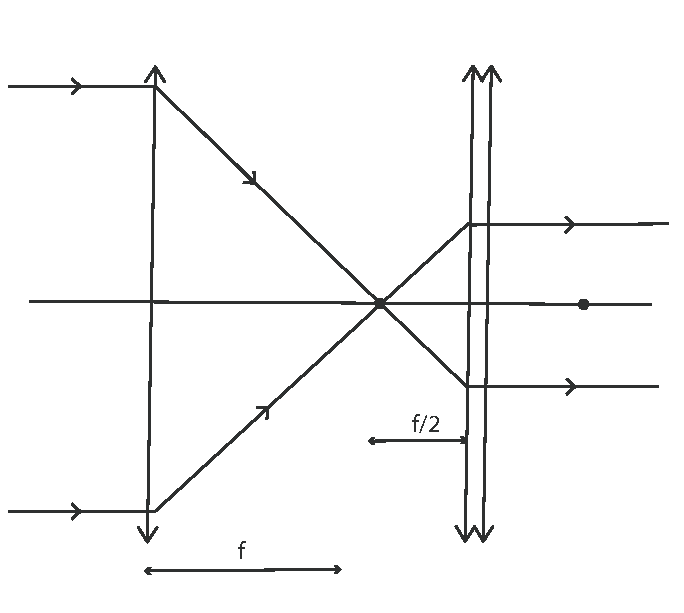
\includegraphics[width=0.45\textwidth]{2020-v2g-10-sol1.pdf}
  \end{center}
  \vspace{-10pt}
  


\emph{Variant 2}\\
\textbf{Teleskoop mis oleks koostatud ühest üksikut läätsest ja ühest kolmeläätselisest komponendist annaks suurenduse 3 korda.}

\vspace{-10pt}
  \begin{center}
    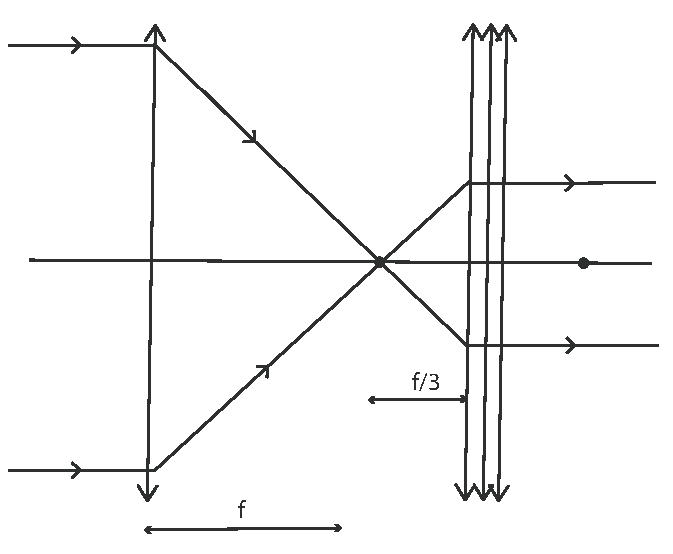
\includegraphics[width=0.45\textwidth]{2020-v2g-10-sol2.pdf}
  \end{center}
  \vspace{-10pt}


\emph{Variant 3}\\
\textbf{Suurema suurenduse saaks aga hoopis kolmekomponendilise  või neljakomponendilise skeemiga.}

Vaaltleme kahte skeemi:

\textbf{kolm lihtläätse järjest}

\vspace{-10pt}
  \begin{center}
    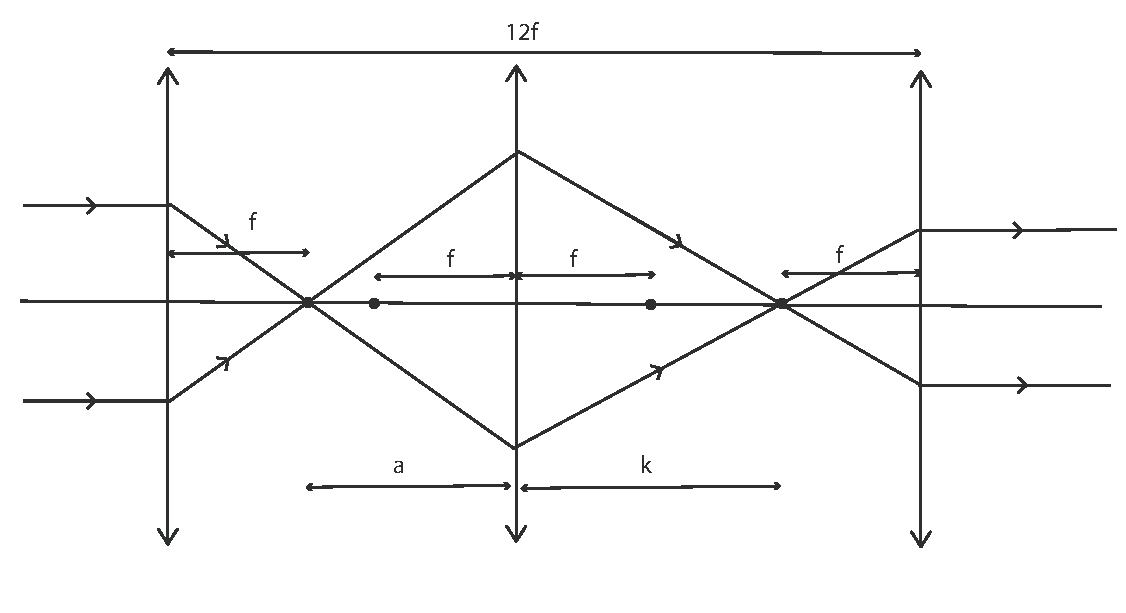
\includegraphics[width=0.8\textwidth]{2020-v2g-10-sol3.pdf}
  \end{center}
  \vspace{-10pt}

\textbf{lihtlääts - kaheläätseline liitlääts - lihtlääts}

\vspace{-10pt}
  \begin{center}
    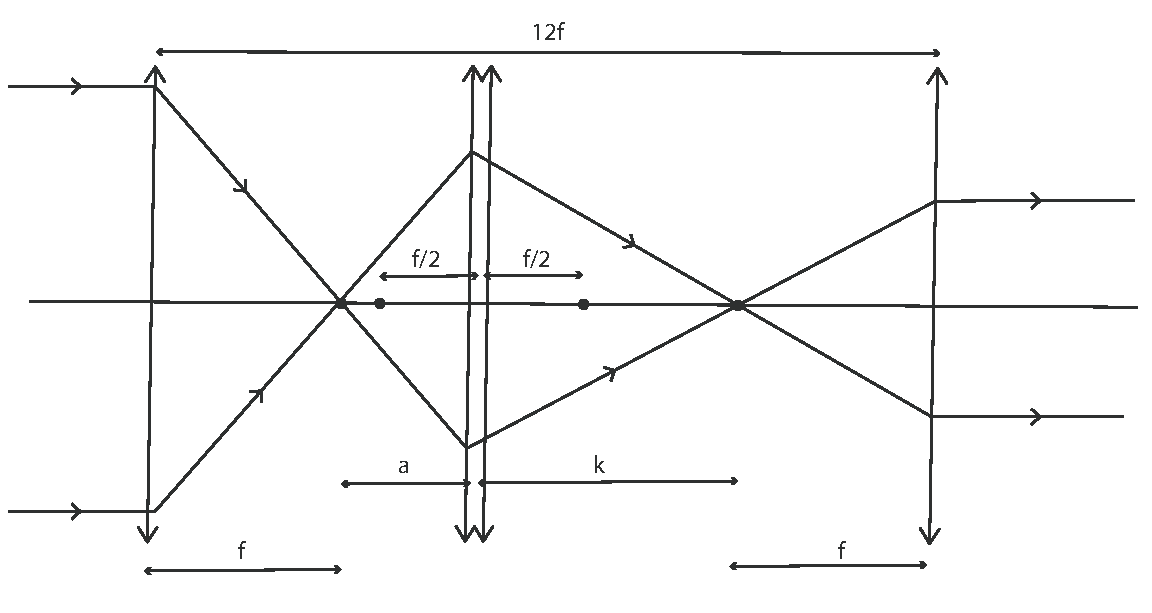
\includegraphics[width=0.8\textwidth]{2020-v2g-10-sol4.pdf}
  \end{center}
  \vspace{-10pt}

Nimelt hakkab keskmine lääts sellise skeemi korral käituma justkui kaks kõrvutiasetatud läätse fookuskaugustega vastavalt $ a $ ja $ k $ .

Süsteemi kogusuurenduseks tuleks sel juhul

 $ {\beta}_{kogu} = {\beta}_1 \cdot {\beta}_2 = \frac {f} {a} \cdot \frac {k} {f} = \frac {k}{a}$

Näeme et parima tulemuse saame kui $a$ oleks võimalikult väike ja $k$ oleks võimalikult suur.

Üheläätselise keskläätse puhul ei saa  $a$ olla väiksem kui $f$ (on sellest natukene suurem).

Kaheläätselise keskläätse puhul ei saa aga $a$ olla väiksem kui $ \frac {f}{2}$ (on sellest natukene suurem).

Samas aga $k$ väärtust piirab vaid süsteemi kogupikkusest tulenev piirang. See on aga mõlema süsteemi jaoks ühesugune (tõsi, kaheläätselise keskkomponendi puhul on sama üldpikkuse korral $k$ $ \frac{f}{2}$ võrra pikem) ning tulenevalt suurenduse valemist annab  suurima suurenduse just kaheläätselise keskkomponendiga süsteem!

\textbf{Seega} asetame üksikläätsed toru otstesse ja topeltläätse esiläätsele võimalikult lähedale nii, et esimese läätse fookuse kujutis tekiks kaksikläätse abil tagumise läätse fookusesse.
Kaheläätselise keskelemendiga süsteemi jaoks saame seosed

$ 12f = f + a + k + f $ ehk $ 10f = a + k $ ehk $ k = 10f - a $

ja

$ \frac{2}{f} = \frac{1}{a} + \frac{1}{k} $

asendame esimese teise

$ \frac {2}{f} = \frac {1}{a} + \frac {1}{10f - a} $

viime ühisele nimetajale, ristkorrutis, jagame miinus kahega, saame ruutvõrrandi

$ a^2 - 10fa + 5f^2 =0 $

mille lahendiks on $ a = (5 \pm \sqrt{20}) f $ kust $a=0.52786f $ ja $k=9.47213f$ .

Maksimaalseks suurenduseks tuleb seega $ {\beta}_{kogu} = 17.944 \approx 18 $ .


\emph{Variant 4}\\
\textbf {Kui kolmekomponendilises süsteemis kasutati siiski vaid üheläätselist keskelementi saame seosed:}

$ 12f = f + a + k + f $ ehk $ 10f = a + k $ ehk $ k = 10f - a $

ja

$ \frac {1}{f} = \frac{1}{a} + \frac{1}{k} $

asendame esimese teise

$ \frac {1}{f} = \frac {1}{a} + \frac {1}{10f - a} $

viime ühisele nimetajale, ristkorrutis, saame ruutvõrrandi

$ a^2 - 10fa + 10f^2 =0 $

mille lahendiks on $ a = (5 \pm \sqrt{15}) f $ kust $a=1.12702f $ ja $k=8.87298f$ .

Maksimaalseks suurenduseks tuleb seega $ {\beta}_{kogu} = 7.872 \approx 8 $ .

\emph{Variant 5}\\
\textbf {Üks variantidest on ka nelja läätsega süsteem:}

Puudusesks on nagu ka kolmest lihtläätsest süsteemi korral sama suurenduse saamiseks vajalik suurem üldpikkus.

\vspace{-10pt}
  \begin{center}
    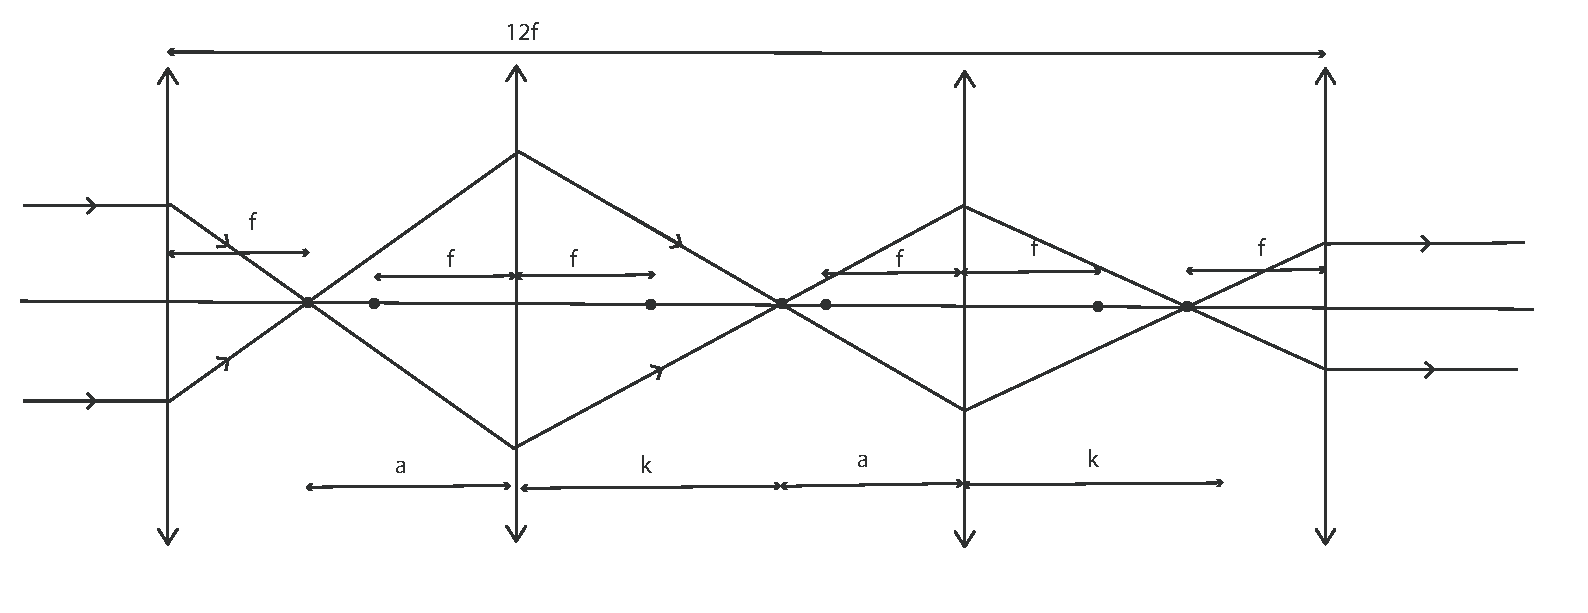
\includegraphics[width=1\textwidth]{2020-v2g-10-sol5.pdf}
  \end{center}
  \vspace{-10pt}


$ 12f = f + a + k + a + f $ ehk $ 5f = a + k $ ehk $ k = 5f - a $

ja

$ \frac {1}{f} = \frac{1}{a} + \frac{1}{k} $

asendame esimese teise

$ \frac{1}{f} = \frac {1}{a} + \frac{1}{5f - a} $

viime ühisele nimetajale, ristkorrutis, saame ruutvõrrandi

$ a^2 - 5fa + 5f^2 =0 $

mille lahendiks on $ a = (2.5 \pm \sqrt{1,25}) f $ kust $a=1.38197f $ ja $k=3.61803f$ .

Maksimaalseks suurenduseks tuleb seekord aga  
\[ {\beta}_{kogu} = {\beta}_1 \cdot {\beta}_2 \cdot {\beta}_3 = \frac {f}{a} \cdot \frac {k}{a} \cdot \frac {k}{f} = {(\frac {k}{a})}^2 = 2.618^2 = 6.854 \approx 7. \]
\probend